\documentclass[11pt]{article}
\usepackage[margin=1in]{geometry}
\usepackage{booktabs}
\usepackage{graphicx}
\usepackage{microtype}
\usepackage[hidelinks]{hyperref}

\newcommand{\IntentAcc}{0.844}
\newcommand{\IntentMacroF}{0.723}
\newcommand{\PolarityAcc}{0.947}
\newcommand{\NTest}{13,521}


\title{\vspace{-2em}\textbf{Experiment 02 — Citation-intent labeling quality}}
\author{arxivkg · preprocessing · phase 3 (label / bert)}
\date{}

\begin{document}
\maketitle
\vspace{-2em}

\section*{What we did}
Phase-3 types every citation edge with an \textbf{intent} (6-way: uses / extends / compares /
motivates / background / critiques) and a \textbf{polarity} (3-way), via a Gemma teacher distilled
into a DistilBERT student. We measure labeling quality in two halves: the teacher prompt's six-round
evolution, and the distilled student's held-out per-class PRF for both heads.

\section*{Method}
Pure reads of frozen artifacts (\texttt{data/models/student-v*/test\_report.json} + the v1--v6
prompts). No model loaded. This is the stage-1 (distilled-label) benchmark; the stage-2 human-gold
benchmark comes from the Phase-C labeling tool.

\section*{Teacher prompt evolution}
\begin{center}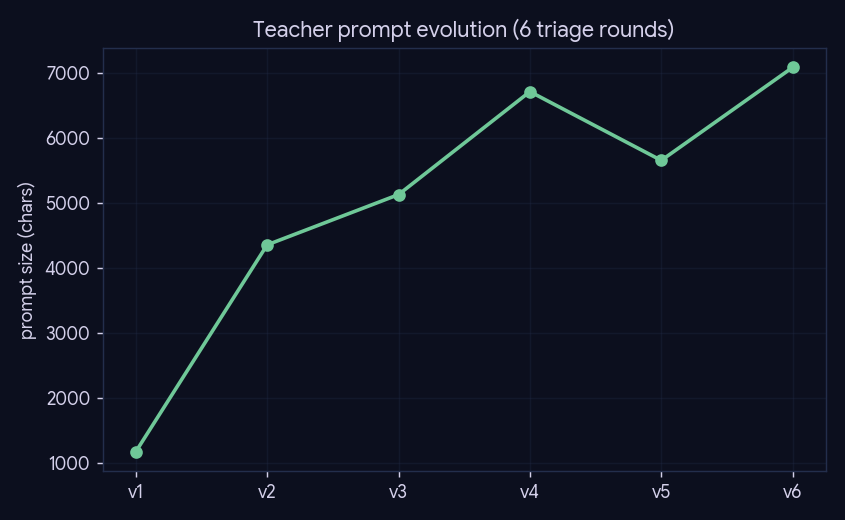
\includegraphics[width=0.62\textwidth]{../results/prompt_growth.png}\end{center}

\section*{Student quality (held-out test, n = \NTest)}
Shipped = \textbf{student-v3}: intent acc \textbf{\IntentAcc} / macro-F1 \textbf{\IntentMacroF},
polarity acc \textbf{\PolarityAcc}.

\begin{center}\begin{tabular}{lrrr}
\toprule
student & intent acc & intent macro-F1 & polarity acc \\
\midrule
student-v1 & 0.894 & 0.717 & 0.962 \\
student-v2 & 0.897 & 0.713 & 0.965 \\
student-v3 & 0.844 & 0.723 & 0.947 \\
\bottomrule
\end{tabular}
\end{center}

\begin{center}
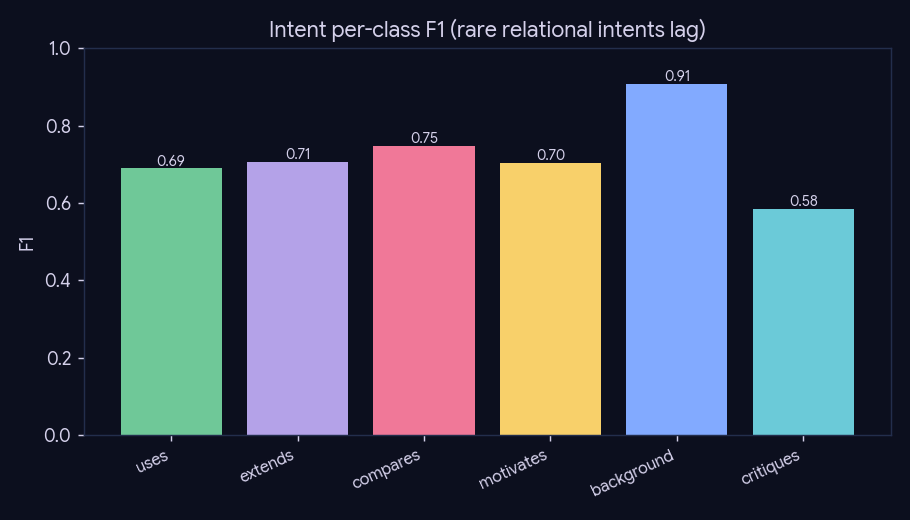
\includegraphics[width=0.62\textwidth]{../results/intent_f1.png}\\
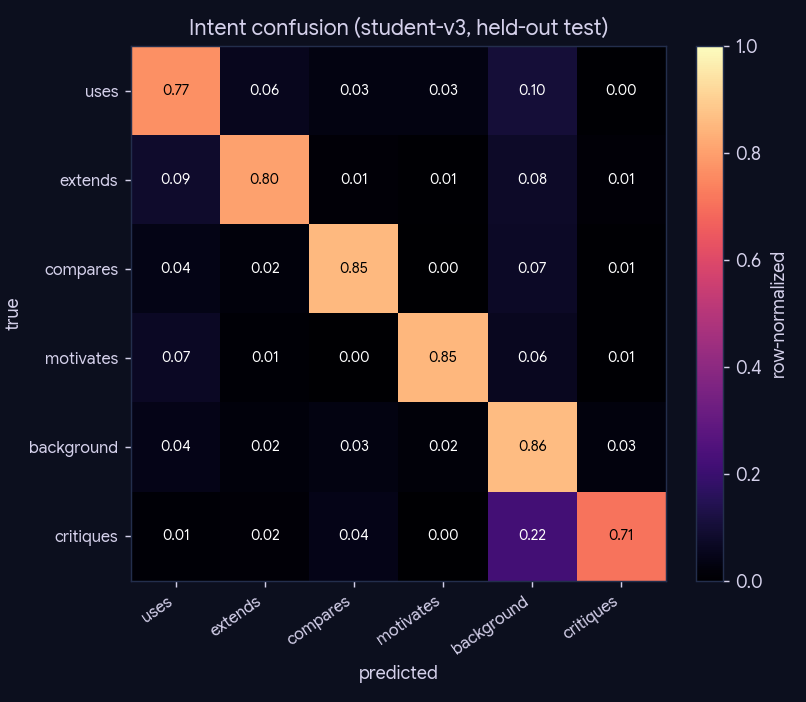
\includegraphics[width=0.55\textwidth]{../results/intent_confusion.png}\\
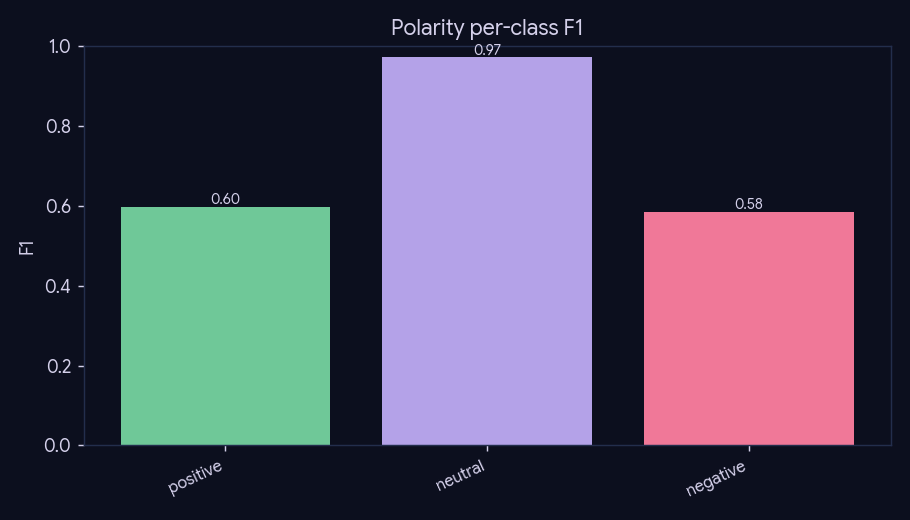
\includegraphics[width=0.62\textwidth]{../results/polarity_f1.png}
\hspace{0.5em}
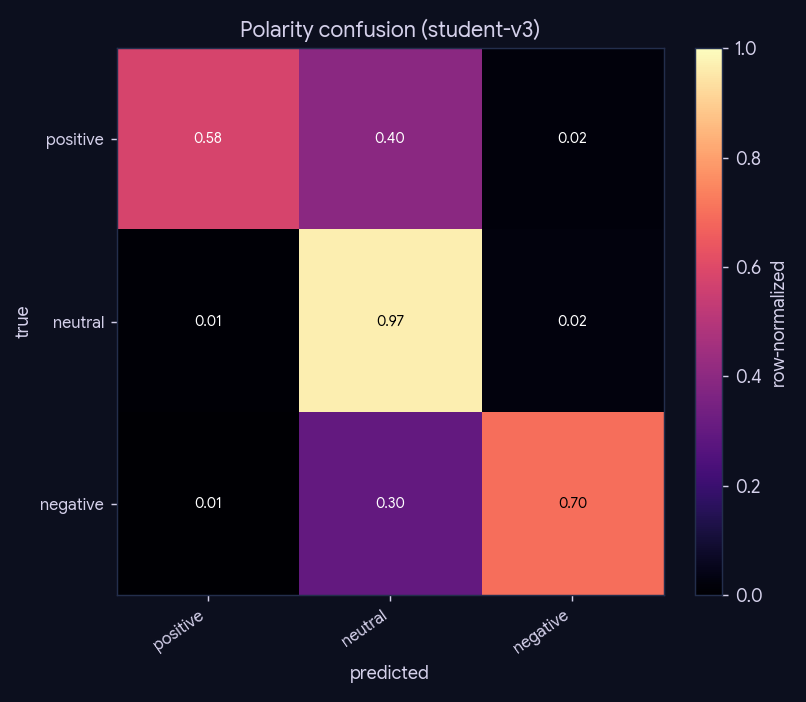
\includegraphics[width=0.40\textwidth]{../results/polarity_confusion.png}
\end{center}

\section*{Conclusion}
Polarity is near-solved (acc 0.95). Intent is strong overall (acc 0.84, macro-F1 0.72) but the rare
relational intents (\texttt{critiques} 0.58; \texttt{motivates}/\texttt{extends}/\texttt{uses}
$\sim$0.70) lag the dominant \texttt{background} (0.91) --- exactly the edge types phase-6's
tensions/open-problems surfacing depends on. macro-F1 $<$ accuracy reflects this class imbalance.
This is a distilled-label benchmark, not human ground truth --- those rare classes are what the
Phase-C human-gold set must validate.

\end{document}
